% give a lot of examples of usages of notebooks in laboratories
% mistakes made then, that will be overcomed with IPython
% the way of writing, connected with IPython again

To clearly understand the problem that this project is trying to solve, we have to go into detail about the concept of using computational applications. The central hypothesis of the research is to analyse over the usage of software in science. However, this area of study wraps great deal of use cases - it can not be measured with general algorithms. A lot of journals and projects that are using coding, would be the evidence and solution of the raised questions - is software helpful for science?; why do we have to use software in analysis?; how a completely different area of study can benefit from the usage of programming scripts? 

\subsection*{Contributions}

Software has contributed to a lot of areas of study.


\subsection*{Approach}

A great deal of researches and journals have been conducted for answering the above questions, which later led to to the idea of observing these investigations in order to assess broadly if software is worth practicing. 

One example for scientifically modeling natural phenomena is the formulation of a snowflake. Norman Packard created the illustration with the use of a program, which demonstrates cellular automation.\cite{wolfram1984computer}\cite{packard1986lattice} The model represents the surface into cells - they have value 0 or 1, which corresponds accordingly to water vapor(black) or to ice(colour). The construction of the model starts with a red cell in the center of the visualisation. Afterwards, it continues by developing series of steps. In order to identify the value of the next cell, the values of the six surrounding cells has to be summed - if it is an odd number, then the cell has to be ice with value 1, if not - the other way around, vapor with value 0. The snowflakes consists of red and blue colours. Its creation requires at least 10,000 calculations. The best possible approach for the accurate and fast generation of the model, was by using computer stimulation. Even if the calculations are simple, the software script helps with the correct build of the pattern.\cite{wolfram1984computer} In figure \ref{fig:snowflake} on page \pageref{fig:snowflake} you can see the snowflake illustration.

\begin{figure}[h]
\centering
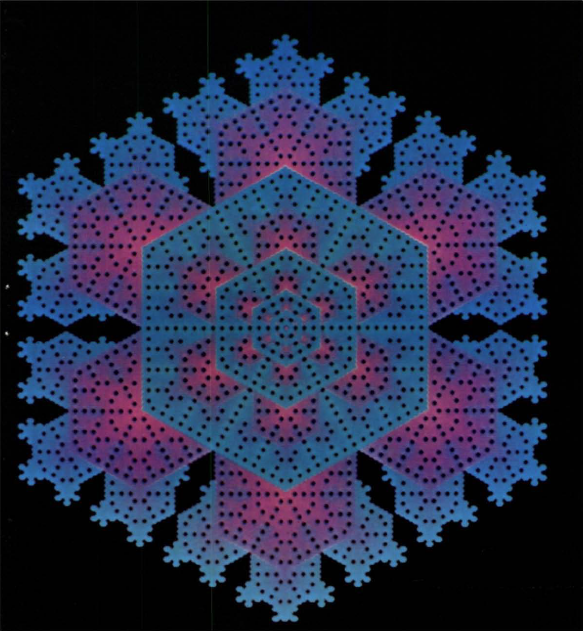
\includegraphics[scale=0.6]{images/snowflake_algorithm}
\caption{Computer Stimulation: Cellular Automation of a snowflake}
\label{fig:snowflake}
\end{figure}

\subsection*{Methodology and Outcomes}

This section explains how we are assessing the usage of software given all of its history in science.

 \cite{chasmSoftware}
